\subsubsection{Fragment show view }

After a new fragment was created, the user could see it in details by clicking on the link of the fragment. The fragment view page shows on the left side the plagiarized text, and on the right side the source. There was also a button to hide/show the colors. If the user hit the button ''Hide color'' the text would be shown with no colors.

There might be a small improvement in comparison with Vroniplag, that the page and the lines of the fragment would be shown here not manually, but automatized.

\begin{figure}[!h]
  \centering
  \fbox{
    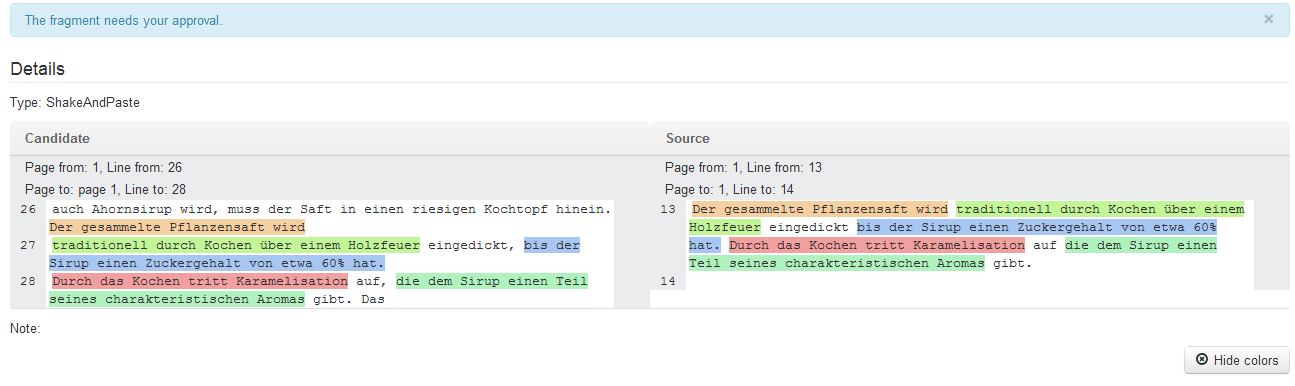
\includegraphics[width=0.97\textwidth]{images/frag_view.png}
  }
  \caption{Text comparison function in fragment show view with colorsr}
  \label{fig:cropping-avatar}
\end{figure}

\begin{figure}[!h]
  \centering
  \fbox{
    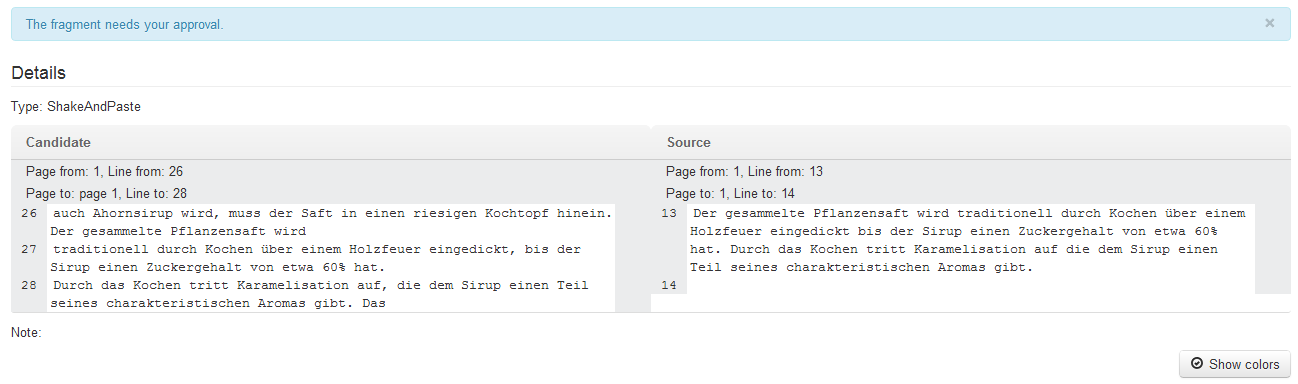
\includegraphics[width=0.97\textwidth]{images/frag_view_plain.png}
  }
  \caption{Text comparison function in fragment show view with no colorsr}
  \label{fig:cropping-avatar}
\end{figure}